\chapter{Plasma Control Systems}

\section{Overview of control systems}
The control of  plasma position, shape and current among other parameters is one of the crucial engineering problems for present and future magnetic confinement devices. The Plasma Control Systems (PCS) lead with the overall control of  fusion devices being responsible also for the  plasma configuration and scenarios algorithms \cite[Chapter~8]{PCS_2018}. Currently different PCS's are use in the tokamaks around the world. In this chapter the "DIII-D-like" PCS, the Syst\'eme de Contr\^ole Distribu\'e (SCD) and the Multi-threaded Application Real-Time executor (MARTe) will be approach, this last one being of special interest due to its extensive utilization in this work.

\subsection{DIII-D Plasma Control System}  

Early documentation regarding the PCS in DIII-D\footnote{DIII-D is a D-shape tokamak operated by General Atomics in San Diego, California. } reefers to digitalization of analog signals transmitted to a high speed processor executing a shape control algorithm and then writing the result to a digital to analog converter for driving the controlled systems . The real-time computer used allowed to performed operations with vectors and matrices required for the plasma shape control algorithm \cite{DIIDcontrol}. Figure ~\ref{DIII1991} shows the block diagram of the DIII-D PCS 30 years ago.
\hfil

\begin{figure}[htbp]
	\centering
	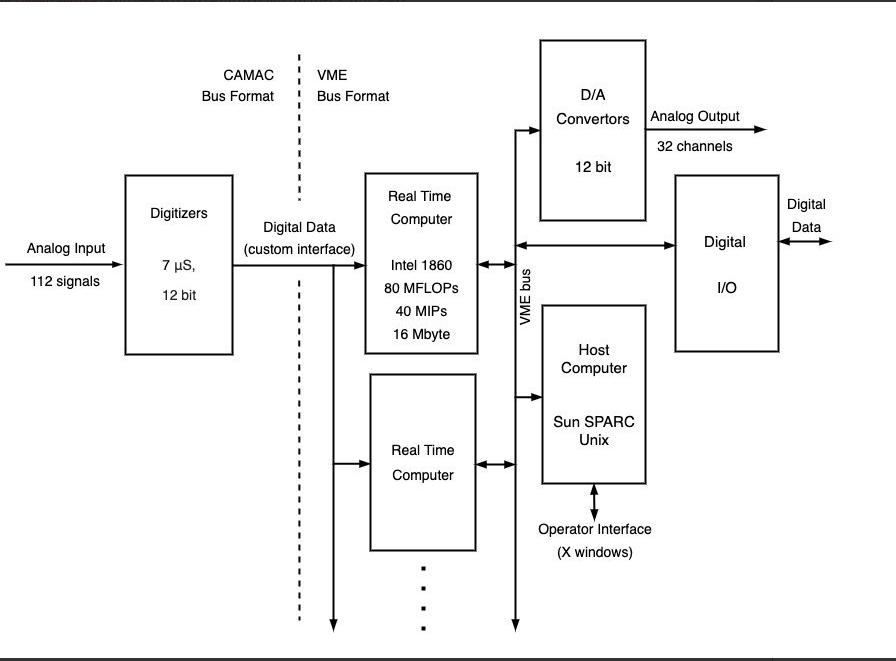
\includegraphics[width=0.65\textwidth]{Chp2/DIIDPCS_old.PNG}
	\caption{\label{DIII1991} DIII-D digital PCS in 1991 ~\cite{DIIDcontrol}.  }
\end{figure}

Blablabla 

\subsection{Syst\'eme de Contr\^ole Distribu\'e}

The TCV distributed control system uses a modular network of real time PC nodes liken by a real time network to provide feedback control over all of the actuator systems. Each node consists of a Linux PC either embedded on a Compact-PCI module or as a desktop computer with Intel CPU. A real time CPU-only node is dedicated to the real time equilibrium reconstruction and fast Fourier transforms for MHD detection.  \cite{TCVcntrl}

\begin{figure}[htbp]
	\centering
	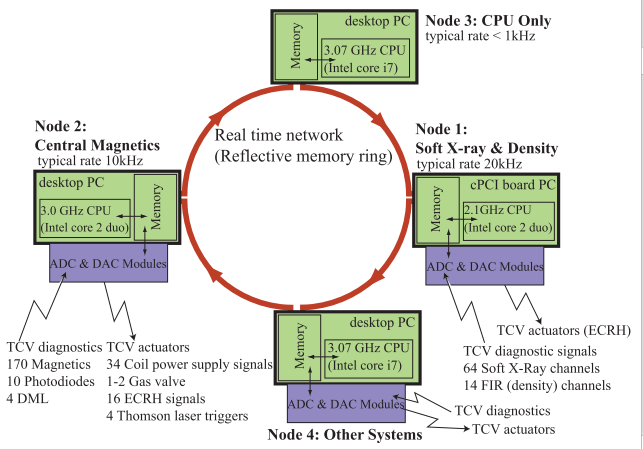
\includegraphics[width=0.65\textwidth]{Chp2/TCVcntrl.png}
	\caption{\label{TCVcontrol} TCV SCD. Real-time network nodes connection. The nodes configurations
		are shown together with the typical diagnostic and actuator systems to which they are connected  ~\cite{TCVcntrl}.  }
\end{figure}

\section{MARTe framework}

MARTe was developed in order to standardize general real-time control systems for the execution of control algorithms. MARTe framework is based on a multiplatform $C^{++}$ library. \cite{Neto2011} 

\subsection{MARTe architecture }
\subsection{Hardware containers}
\subsection{MARTe 2.0}
\section{Equilibrium and control algorithms} 
\subsection{PID control}
\subsection{Multiple-Input Multiple-Output control}